\begin{tikzpicture}
	\vspace*{3cm}
	\onslide<1>{
		\node(img) at (0,0.6){
			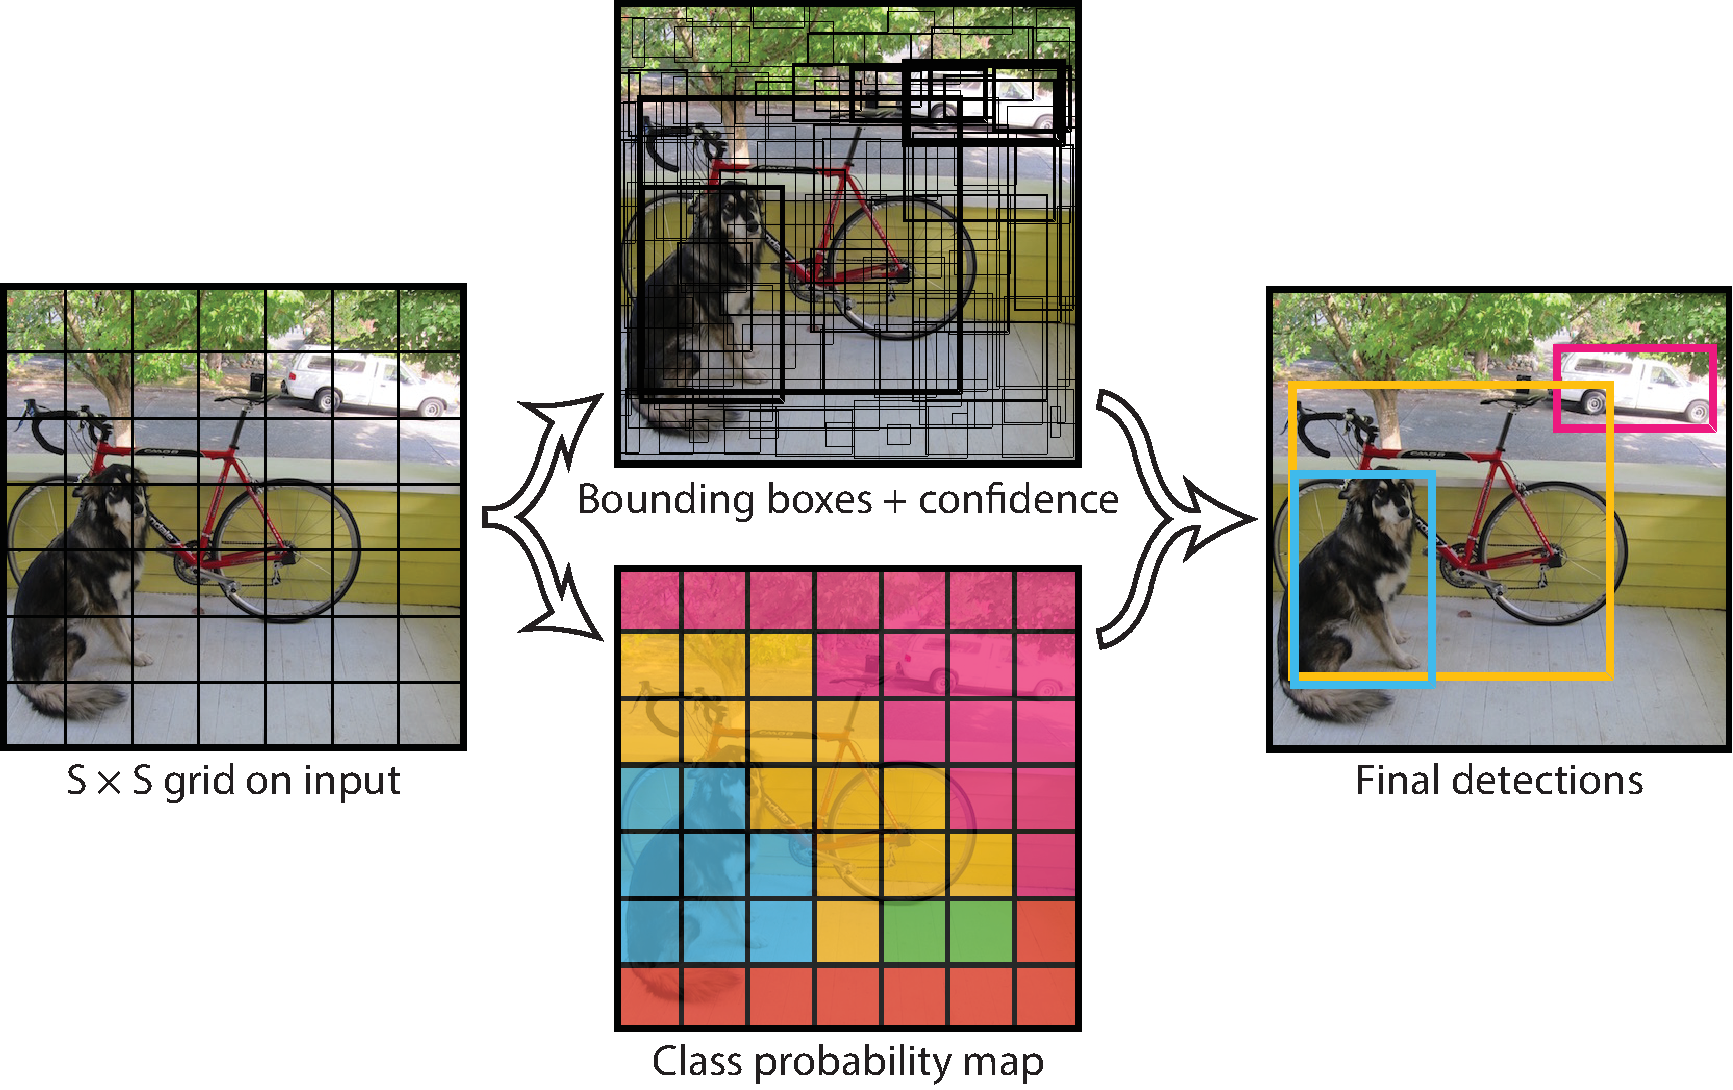
\includegraphics[scale=0.4,trim={0cm 5.6cm 21.5cm 3cm},clip]{images/dog.pdf}        
		};    
		\node(label) at (0,-1.8){\footnotesize Input Image};
	}
	\onslide<2-10>{
		\node(img) at (0,0.15){
			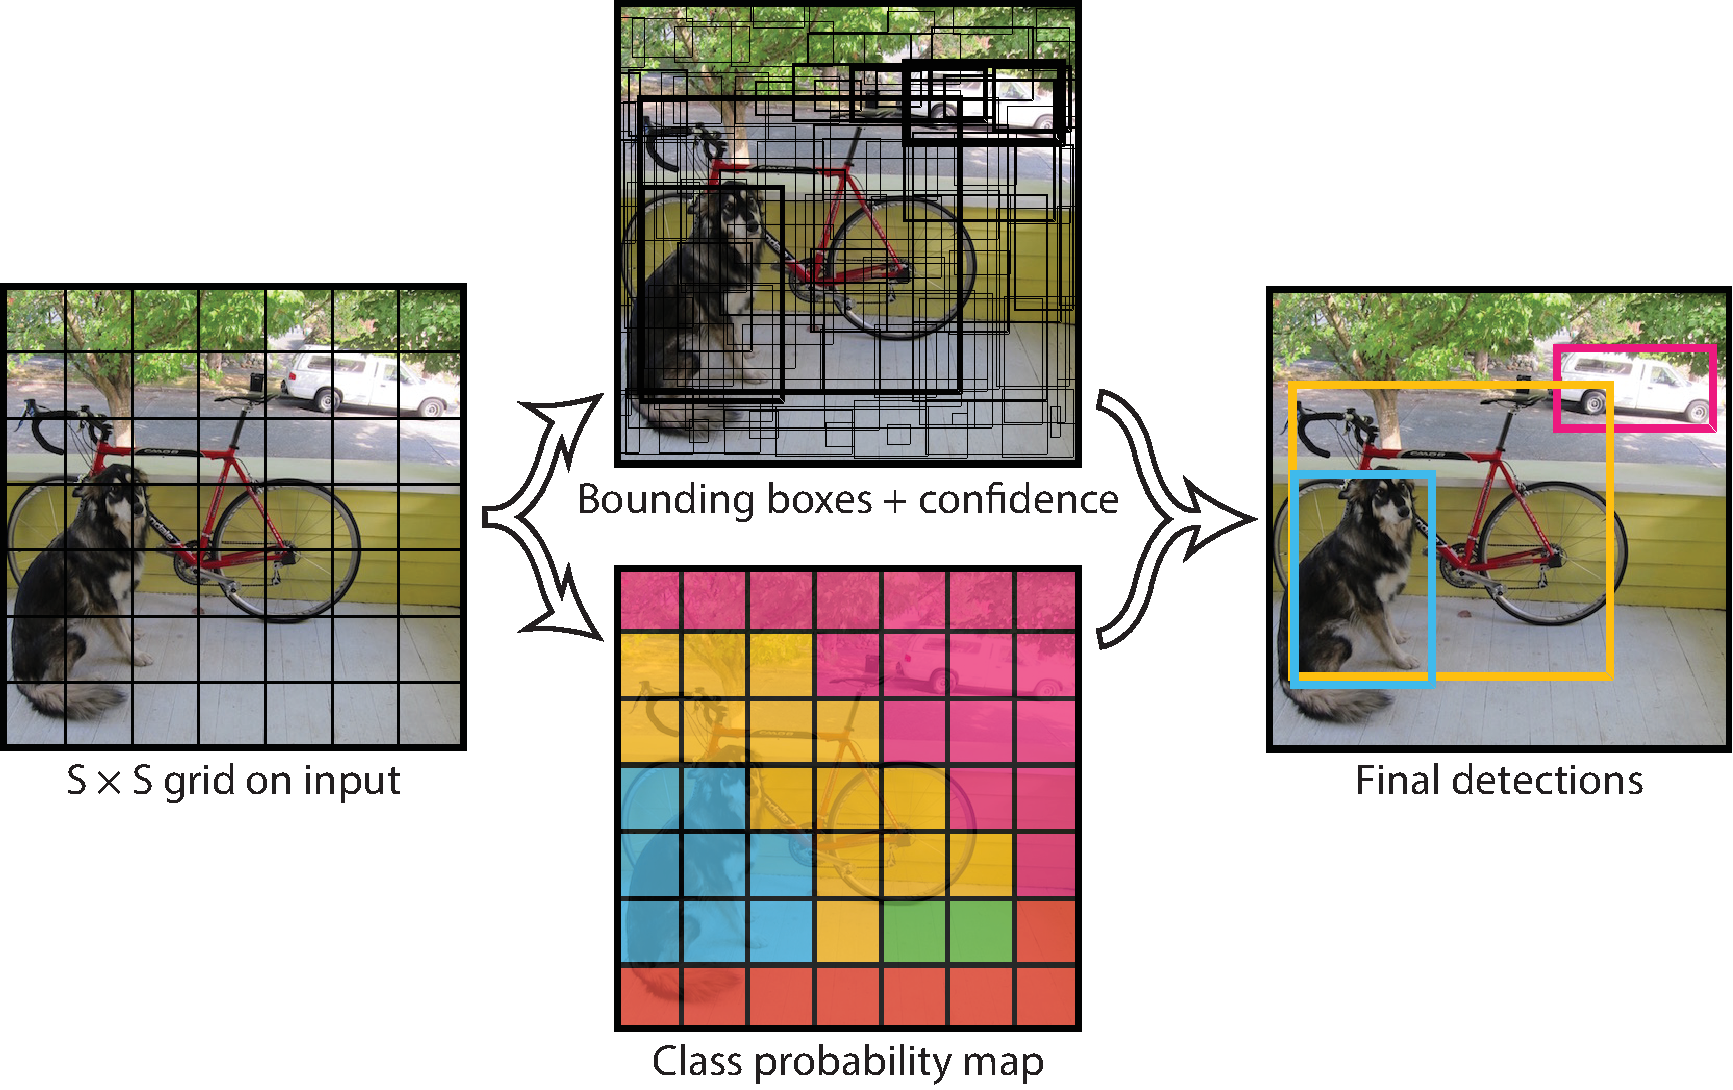
\includegraphics[scale=0.4,trim={0cm 4.5cm 21.2cm 4cm},clip]{images/dog.pdf}
		};
		\pgfmathsetmacro\x{-1.2}
		\pgfmathsetmacro\y{-0.45}
		\filldraw[fill=cyan!80, draw=cyan,opacity=0.5](\x,\y) rectangle (\x+0.48,\y+0.48);
	}
	\onslide<3-10>{
		\draw[line width=0.7mm,color=cyan] (-1.4,-0.9) rectangle (-0.5,0.6);  
	}

	\onslide<4-10>{
		\pgfmathsetmacro\x{0.6}
		\pgfmathsetmacro\y{-0.9}
		\filldraw[fill=green!70, draw=black,opacity=0.5](\x,\y) rectangle (\x+0.48,\y+0.48);
	}
	\onslide<5-10>{
		\draw[line width=0.2mm,color=green,dashed] (0.2,-1.2) rectangle (1.5,-0.12);  
	}
	\onslide<6-10>{
		\pgfmathsetmacro\x{-0.75}
		\pgfmathsetmacro\y{0}
		\filldraw[fill=yellow!70, draw=black,opacity=0.5](\x,\y) rectangle (\x+0.48,\y+0.48);
	}
	\onslide<7-10>{
		\draw[line width=0.1mm,color=yellow,line width=0.7mm] (-1.4,-0.8) rectangle (0.7,1.2);  
   
	}

	\onslide<8-10>{
		\pgfmathsetmacro\x{0.6}
		\pgfmathsetmacro\y{0.9}
		\filldraw[fill=magenta!70, draw=black,opacity=0.5](\x,\y) rectangle (\x+0.48,\y+0.48);
	}
	\onslide<9-10>{
		\draw[line width=0.1mm,color=magenta,line width=0.7mm] (0.3,0.8) rectangle (1.5,1.5); 

	}

	\onslide<10>{
		
		\pgfmathsetseed{1}
		\foreach \x in {-0.8,-0.5,...,0.8}{
			\foreach \y in {-0.8,-0.4,...,0.8}{
				\draw[red!50,dashed] (\x+rand,\y)rectangle (\x+rand,\y+rand);       
			}
		}     
		

		\draw[red,dashed] (0,0.15)rectangle (0.5,0.5);
		
		\node(label) at (0,-2.3){\footnotesize Bounding Boxes \& Confidence};
	}
	

	\onslide<11->{
		\node(img) at (0,1.2){
			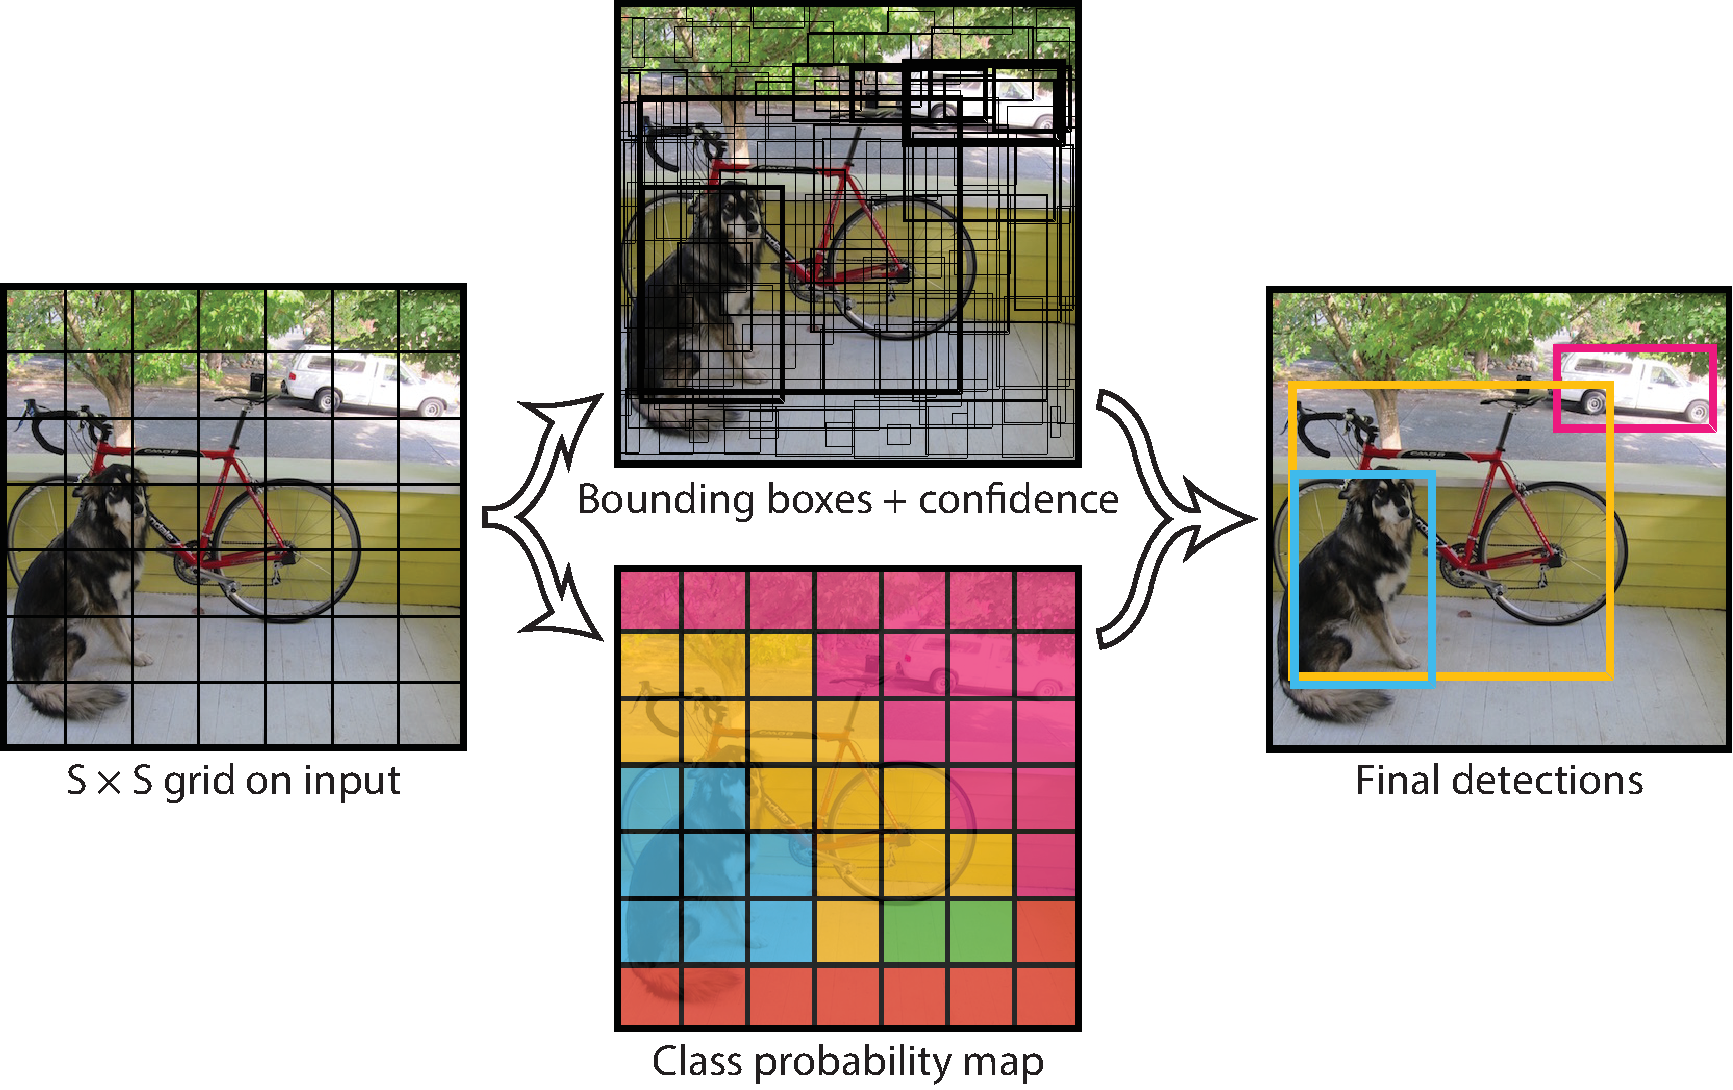
\includegraphics[scale=0.41,trim={21.5cm 5.6cm 0cm 0cm},clip]{images/dog.pdf}
		};
		%     \node(label) at (0,-2){\footnotesize Final Detection};
	}
\end{tikzpicture}
